\documentclass[../Relazione.tex]{subfiles}

\begin{document}

\section{Accessibilità}

\subsection{Separazione tra contenuto-struttura-presentazione}

Per migliorare l'accesso al sito agli utenti con differenti disabilità e ai motori di ricerca è stata mantenuta la separazione tra struttura, presentazione e comportamento. La prima è stata sviluppata tramite documenti XHTML Strict 1.0, i quali richiamano i fogli di stile esterni CSS che implementano la presentazione e script esterni realizzati con JavaScript che formano il comportamento. Questi script sono stati implementati in modo da garantire una trasformazione elegante del sito, poiché se JavaScript è disabilitato il contenuto rimane comunque accessibile. Tutto il codice redatto è stato scritto secondo le raccomandazioni W3C, accertando che fossero state rispettate tramite validazione.

\subsection{Schema colori}

Si è cercato di utilizzare uno schema colori tale che garantisca un contrasto elevato, in modo da facilitare la lettura del contenuto anche alle persone con disturbi visivi. Inoltre, i link vengono sempre rappresentati sottolineati e rispettando sempre la convenzione interna del sito. Per garantire che il sito sia accessibile anche alle persone con disturbi visivi è stato utilizzato il servizio offerto dal sito \url{http://www.color-blindness.com/coblis-color-blindness-simulator/} che a partire da uno screenshot di una pagina, mostra come viene visualizzata da persone con determinati disturbi visivi. Viene di seguito riportato il risultato ottenuto dal test della homepage.
\newpage

\begin{figure}[!h]
		\centering
		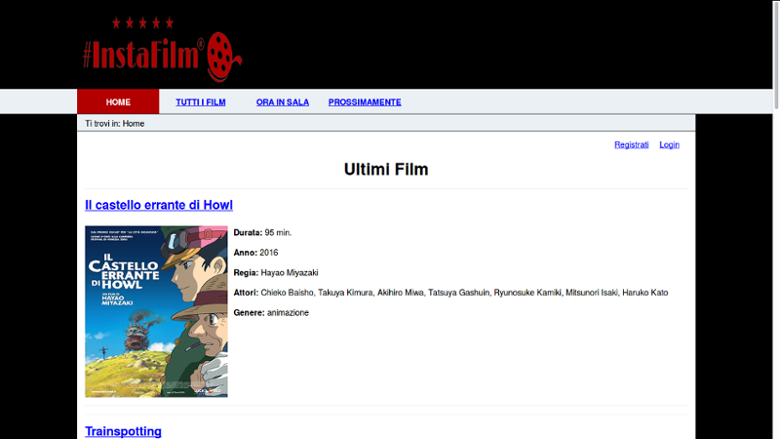
\includegraphics[scale=0.4]{immagini/prova.png}
			\caption{Homepage del sito}
		\label{fig:Homepage del sito}
\end{figure}

\begin{figure}[!h]
		\centering
		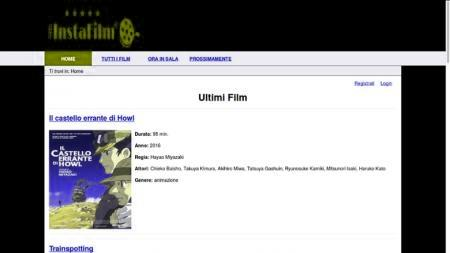
\includegraphics[scale=0.7]{immagini/prova_deuteranopia.jpg}
			\caption{Homepage del sito - Deuteranopia}
		\label{fig:Homepage del sito}
\end{figure}

\begin{figure}[!h]
		\centering
		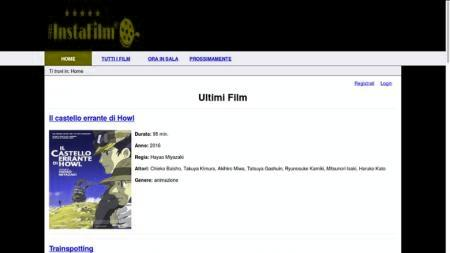
\includegraphics[scale=0.7]{immagini/prova_protanopia.jpg}
			\caption{Homepage del sito - Protanopia}
		\label{fig:Homepage del sito}
\end{figure}

\begin{figure}[!h]
		\centering
		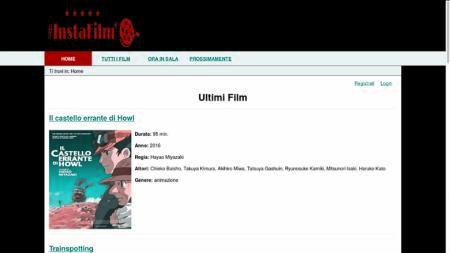
\includegraphics[scale=0.7]{immagini/prova_tritanopia.jpg}
			\caption{Homepage del sito - Tritanopia}
		\label{fig:Homepage del sito}
\end{figure}

\newpage
\subsection{Utilizzo dei tag}

Sono stati inseriti per ogni pagina i tag \textit{meta}: \textit{Content-Type}, \textit{keywords}, \textit{description}, \textit{author} e \textit{languages} e il tag \textit{title}, il quale descrive la pagina corrente \textbf{dal particolare al generale}. Il tag \textit{languages} indica che il sito è stato interamente scritto in italiano ma compaiono alcune parole inglesi, le quali sono state affiancate dall’attributo: \textit{xml:lang=”en”}.

\subsection{Screen reader}

Ogni locandina è stata arricchita di attributi \textit{alt} e \textit{title} che descrivono in maniera esaustiva ciò che l'immagine ritrae. Per le immagini che sono state ritenute non di contenuto, e che sono così state inserite tramite CSS, non è stato previsto l'uso di questi attributi, poiché la loro unica funzione è di presentazione, non portando valore aggiunto al contenuto.
Ogni campo di un form è stato sempre corredato con una etichetta \textit{label}.

\subsection{Aiuti per la navigazione}

Al fine di aumentare l'accessibilità del sito sono previsti le seguenti facilitazioni per la navigazione:

\begin{itemize}
\item \textbf{Colori dei link}: per evitare il disorientamento durante la navigazione, sono previsti colori differenti per i link attivi visitati (\textbf{blue}) e quelli non visitati (\textbf{viola});
\item \textbf{Tabindex}: ad ogni pressione del tasto tab il focus si sposta sul link direttamente successivo per agevolare la navigazione. Sono stati ridefiniti gli attributi \textit{tabIndex} dei link in modo da rispecchiare l'ordine desiderato;
\item \textbf{Link per spostarsi al contenuto}: prima del menù di navigazione è stato inserito un link, nascosto all'utenza normale, ma che permette agli utenti che visualizzano il sito mediante uno screen reader di saltare la barra di navigazione;
\item \textbf{Link per tornare al menù}: Per facilitare la navigazione nel sito sono stati creati dei link interni alla pagina che permettono agli utenti di tornare al menù di navigazione.

\end{itemize}

\end{document}
